\documentclass{article}
\usepackage{tikz}
\usetikzlibrary{calc,shapes.multipart,chains,arrows}

\begin{document}

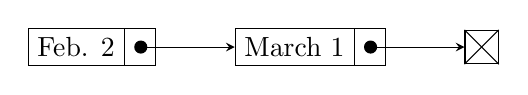
\begin{tikzpicture}[list/.style={rectangle split, rectangle split parts=2,
    draw, rectangle split horizontal}, >=stealth, start chain]

  \node[list,on chain] (A) {Feb. 2};
  \node[list,on chain] (B) {March 1};
  \node[on chain,draw,inner sep=6pt] (E) {};

  \draw (E.north east) -- (E.south west);
  \draw (E.north west) -- (E.south east);

  \draw[*->] let \p1 = (A.two), \p2 = (A.center) in (\x1,\y2) -- (B);
  \draw[*->] let \p1 = (B.two), \p2 = (B.center) in (\x1,\y2) -- (E);

\end{tikzpicture}

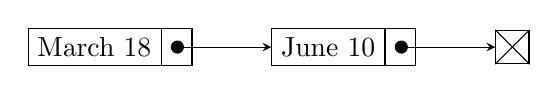
\begin{tikzpicture}[list/.style={rectangle split, rectangle split parts=2,
    draw, rectangle split horizontal}, >=stealth, start chain]

  \node[list,on chain] (C) {March 18};
  \node[list,on chain] (D) {June 10};
  \node[on chain,draw,inner sep=6pt] (E) {};

  \draw (E.north east) -- (E.south west);
  \draw (E.north west) -- (E.south east);

  \draw[*->] let \p1 = (C.two), \p2 = (C.center) in (\x1,\y2) -- (D);
  \draw[*->] let \p1 = (D.two), \p2 = (D.center) in (\x1,\y2) -- (E);

\end{tikzpicture}

\end{document}